\documentclass[supercite]{HustGraduPaper}
%进行个人信息设置
\title{植物图像抠图方法复现与对比} %论文题目
\author{\small{李新利($100\%$)}} %作者姓名
\date{\today} %日期，默认当日
\school{人工智能与自动化学院} %院系名称
\classnum{自动化2001班} %专业班级
\stunum{\small{U202012345}} %学号
\instructor{陆昊} %指导教师姓名

%添加自己要用的其他宏包
\usepackage{xltxtra}
\usepackage{bm}
\usepackage{amsfonts}
\usepackage{amsmath,bm}
\usepackage{array}
\usepackage{natbib}
\usepackage{hyperref}
\usepackage{algorithm}
\usepackage{multirow}
\usepackage{bbding}
\usepackage{algorithmic}
\usepackage{mathrsfs,tabularx,multirow,makecell,setspace,subfig,color,booktabs,multirow}
\usepackage{graphicx}
\usepackage{abstract}
\graphicspath{{figures/}}
\definecolor{mygreen}{RGB}{90,135,109}
\renewcommand{\algorithmicrequire}{\textbf{输入:}}
\renewcommand{\algorithmicensure}{\textbf{输出:}}

\begin{document}
	%生成标题页
	\maketitle

	\clearpage %结束上一页
	\pagenumbering{Roman} %摘要页码为大写罗马数字

	%填写中文摘要内容和关键字
	\begin{cnabstract}{图像抠图；深度学习；植物图像；方法复现}
		图像抠图旨在预测图像中每个像素的前景透明度（alpha matte），从而将目标从背景中自然分离出来，是图像编辑与视觉认知中的一项基础任务。近年来，基于深度学习与大规模预训练模型的抠图方法取得了显著进展。本文面向植物图像这一具体场景，在统一评测协议下复现并对比了四种范式迥异的代表性方法：基于三分图（trimap）精修的 ViTMatte、零样本可提示的 ZIM、扩散式的 SDMatte，以及自动与交互统一的 SMat。所有模型在 PM 植物数据集（150 张，统一缩放至 $1024^2$）上以完全相同的真值与统一三分图评测，同时报告全图与未知（Unknown）区域两套 SAD/MSE/MAD 指标。实验表明：在给定三分图先验时，ViTMatte 取得最佳的全图精度（SAD 25.5）；在三种无三分图方法中，扩散式 SDMatte 表现最稳健（全图 SAD 44.3、零图形-背景反转）。我们进一步在各模型原始论文基准（AIM-500、MicroMat-3K）上做了跨数据集自验，结果与原文趋势一致，确认复现忠实；据此说明植物场景下的较高误差主要源于数据域特性（主体满框、类内相似干扰）而非模型本身。
	\end{cnabstract}
	%填写英文摘要内容和关键字
	\begin{enabstract}{Image Matting; Deep Learning; Plant Images; Reproduction}
		Image matting aims to predict the per-pixel foreground opacity (alpha matte) of an image so as to naturally separate the target from the background, which is a fundamental task in image editing and visual cognition. Recently, matting methods based on deep learning and large-scale pre-trained models have achieved remarkable progress. Focusing on the specific scenario of plant images, this report reproduces and compares four matting methods of distinct paradigms under a unified protocol: trimap-based ViTMatte, zero-shot promptable ZIM, diffusion-based SDMatte, and SMat that unifies automatic and interactive matting. All models are evaluated on the PM plant dataset (150 images resized to $1024^2$) against identical ground truth and a unified trimap, reporting SAD/MSE/MAD over both the whole image and the unknown region. With a trimap prior, ViTMatte attains the best whole-image accuracy (SAD 25.5); among the three trimap-free models, the diffusion-based SDMatte is the most robust (whole-image SAD 44.3, zero figure-ground inversion). Cross-dataset sanity checks on the original benchmarks (AIM-500, MicroMat-3K) match the trends reported in the source papers, confirming faithful reproduction and indicating that the higher error on plants stems from domain characteristics (full-frame subjects, intra-class distractors) rather than the models themselves.
	\end{enabstract}

	%生成目录
	\tableofcontents

	\clearpage%结束上一页
	\pagenumbering{arabic} %正文页码为阿拉伯数字

	\section{引言}
	图像抠图是计算机视觉中的一项基础任务，给定一张 RGB 图像，抠图通过预测前景蒙版（alpha matte）将目标前景从背景中分离出来。早期的深度抠图工作以 DIM~\cite{DIM} 为代表，构建了端到端的预测框架；随后 GCA~\cite{GCA}、IndexNet~\cite{index} 等在网络结构与上采样算子上不断改进。这一类方法大多需要人工提供三分图（trimap）以指明确定前景、确定背景与待求的未知区域。近年来，随着大规模预训练视觉模型（如 SAM~\cite{sam}、DINOv2~\cite{dinov2}、Stable Diffusion~\cite{ldm}）的兴起，出现了一批\emph{无需三分图}的抠图范式：它们借助预训练表征自主完成前景识别与图形-背景分离，或仅依赖点/框等弱提示。

	本文聚焦植物图像这一具体场景。植物主体常呈现细茎、叶尖、绒毛等大量细结构，且常出现主体满框、与背景同种植株相似等困难，对抠图方法的细节感知与图形-背景分离能力构成针对性考验。从视觉认知的角度看，抠图过程隐含了「任务驱动的目标选择」「图形-背景分离」「局部细节注意」等若干基本机制：抠图方法是否需要外部三分图来指明目标，正对应人类视觉中前景是被「自上而下给定」还是「自主从场景中分离」。植物场景中前景与背景常同质，恰好放大了这些机制上的差异，使其成为对照不同抠图范式的良好试验台。

	基于此，本文在统一评测协议下复现并对比四种范式迥异的代表性方法——三分图精修的 ViTMatte~\cite{vitmatte}、零样本可提示的 ZIM~\cite{zim}、扩散式的 SDMatte~\cite{sdmatte}、自动与交互统一的 SMat~\cite{smat}。我们围绕「\textbf{给定前景下的精修}」与「\textbf{自主前景选择}」两条技术路线设计对照实验，在 PM 植物数据集上以完全一致的真值与统一三分图评测，并辅以各模型原始基准上的跨数据集自验以确认复现忠实。本文的工作可概括为：(1) 统一协议下四种范式的可比定量评测；(2) 全图与未知区域双口径指标，分离「前景判定」与「边缘细节」两类误差；(3) 跨数据集自验，论证植物场景误差主要源于数据域而非模型本身。

	\section{相关工作与模型原理}
	早期深度抠图方法（如 DIM~\cite{DIM}、GCA~\cite{GCA}、IndexNet~\cite{index}）在结构与上采样算子上不断改进，但普遍依赖人工三分图来界定前景/背景/未知区域。近年大规模预训练模型催生了一批无需三分图的范式。本文选取的四个 baseline 覆盖了四种典型前端机制——三分图精修、SAM 式零样本可提示、扩散式、自动与交互统一，其\textbf{核心差异在于「前景如何被确定」}：ViTMatte 依赖外部给定的三分图，其余三者则以不同机制自主或弱监督地确定前景。下面分别概述其原理。

	\subsection{ViTMatte：三分图精修}
	ViTMatte~\cite{vitmatte} 以一个朴素的预训练视觉 Transformer（ViT）为骨干，输入为 RGB 图与三分图的拼接，通过轻量的卷积细节捕获模块在未知区域回归 alpha。它不进行前景判定，而是在\emph{已给定}的确定前景/背景约束下做精修，因而作为「给定前景下的精修能力」这一控制变量参与对比。

	\subsection{ZIM：零样本可提示抠图}
	ZIM~\cite{zim} 在 SAM~\cite{sam} 的可提示分割框架上引入层级像素解码器与提示感知掩码注意力，把分割标签转化为细粒度 matte 标签训练，从而在保持零样本能力的同时输出软边缘。推理时接受点/框等视觉提示。本文采用「真值框 + 8 个最远点采样前景点」的弱监督提示协议（信息对等地由真值派生，不手工点击）。

	\subsection{SDMatte：扩散式抠图}
	SDMatte~\cite{sdmatte} 将预训练的 Stable Diffusion 2~\cite{ldm} U-Net 作为先验骨干，把视觉提示（点/框/掩码）注入交叉注意力以驱动前景选择，借助扩散模型强大的纹理与边缘先验生成 alpha。本文使用真值框作为提示（与 ZIM 对齐），单步推理。

	\subsection{SMat：自动与交互统一}
	SMat~\cite{smat} 以预训练 DINOv2~\cite{dinov2} 为骨干，通过提示交叉注意力与细节捕获解码器，将\emph{自动}（无提示，借类别 token 作查询）与\emph{交互}（点/框提示）两种模式统一到同一模型。其训练采用自动与交互混合，使单一模型对两种使用方式均鲁棒。本文同时评测其自动模式（none）与交互模式（8 个真值派生点）。

	\section{数据集与评测协议}
	\subsection{数据集与划分}
	评测在 PM 植物数据集上进行，共 150 对「图像-真值 alpha」，统一缩放至 $1024\times1024$ 以使随像素数缩放的 SAD 在图间、模型间可比。所选 baseline 均为预训练/零样本模型，不存在训练泄漏，故 headline 指标在全部 150 张上报告以最大化评测信号。该数据集部分真值背景存在压缩伪影（背景值为 $2/3/5$ 而非 $0$），若不清洗会使三分图几乎全为未知区域、严重扭曲指标，故先做背景清洗再统一生成三分图（膨胀/腐蚀，未知区灰度 128）。

	\subsection{指标与公平性}
	我们报告 SAD、MSE、MAD 三项主指标，并加报衡量边缘锐度的 Grad 与衡量主体完整性的 Conn；每项均同时给出\textbf{全图（whole）}与\textbf{未知区域（Unknown）}两套数值：前者反映整体前景判定（含图形-背景分离是否正确），后者聚焦边缘细节质量。所有模型在\textbf{完全相同}的清洗后真值与同一套统一三分图下评测，从而让无三分图方法也能与 ViTMatte 在相同区域被公平比较。

	\subsection{实验设计:两条对照轴}
	需强调各模型\textbf{输入条件存在差异}——ViTMatte 享有三分图先验，其余三者没有——故不能简单宣称「ViTMatte 最好」，该差异本身即是分析的切入点。据此本文设计两条对照轴：一是「\textbf{给定前景的精修}（ViTMatte）vs 自主前景选择（其余三者）」，考察前景是否需要外部给定；二是在无三分图方法内部比较「SAM 自动 / 扩散 / 自动+交互」三种前端机制的图形-背景分离鲁棒性。为公平起见，ZIM/SDMatte/SMat 的提示一律由真值\emph{程序化派生}（如真值框、真值最远点采样，信息对等而非手工点击），不引入额外人工监督。

	\section{Baseline 评测结果}
	\subsection{总体指标对比}
	表~\ref{tab:pm} 给出各模型在 PM 数据集上的统一评测结果（全图与 Unknown 双口径，各 5 指标），图~\ref{fig:qual} 给出代表样本的定性对比。

	% Auto-generated by scripts/generate_table.py -- do not edit by hand.
\begin{table}[ht]
\centering
\caption{四个 baseline 在 PM 植物数据集（150 张，$1024^2$）上的统一评测，同时报告全图与 Unknown 区域的 SAD/MSE/MAD/Grad/Conn。所有指标越小越好；MSE/MAD 在 $[0,1]$ 上计算。}
\label{tab:pm}
\small
\setlength{\tabcolsep}{4pt}
\textbf{(a) 全图 (whole)}\\[2pt]
\begin{tabular}{llccccc}
\toprule
模型 & 范式 & SAD & MSE & MAD & Grad & Conn \\
\midrule
ViTMatte-B & trimap 精修 & 25.13 & 0.011 & 0.024 & 76.87 & 15.93 \\
ZIM-L & SAM 自动 (promptable) & 93.23 & 0.075 & 0.089 & 106.08 & 27.96 \\
SDMatte & 扩散 (SD2 先验) & 44.32 & 0.032 & 0.042 & 122.27 & 16.55 \\
SMat-auto & 自动 (DINOv2) & 64.12 & 0.050 & 0.061 & 138.89 & 24.14 \\
SMat-point8 & 交互 (8 点) & 63.31 & 0.049 & 0.060 & 135.54 & 21.97 \\
\bottomrule
\end{tabular}
\\[6pt]
\textbf{(b) Unknown 区域}\\[2pt]
\begin{tabular}{lccccc}
\toprule
模型 & SAD & MSE & MAD & Grad & Conn \\
\midrule
ViTMatte-B & 24.05 & 0.063 & 0.142 & 75.93 & 15.17 \\
ZIM-L & 35.80 & 0.143 & 0.204 & 102.15 & 16.81 \\
SDMatte & 23.91 & 0.097 & 0.139 & 102.14 & 11.29 \\
SMat-auto & 32.84 & 0.140 & 0.186 & 115.22 & 13.37 \\
SMat-point8 & 31.65 & 0.137 & 0.183 & 112.20 & 13.00 \\
\bottomrule
\end{tabular}
\end{table}


	\begin{figure}[ht]
		\centering
		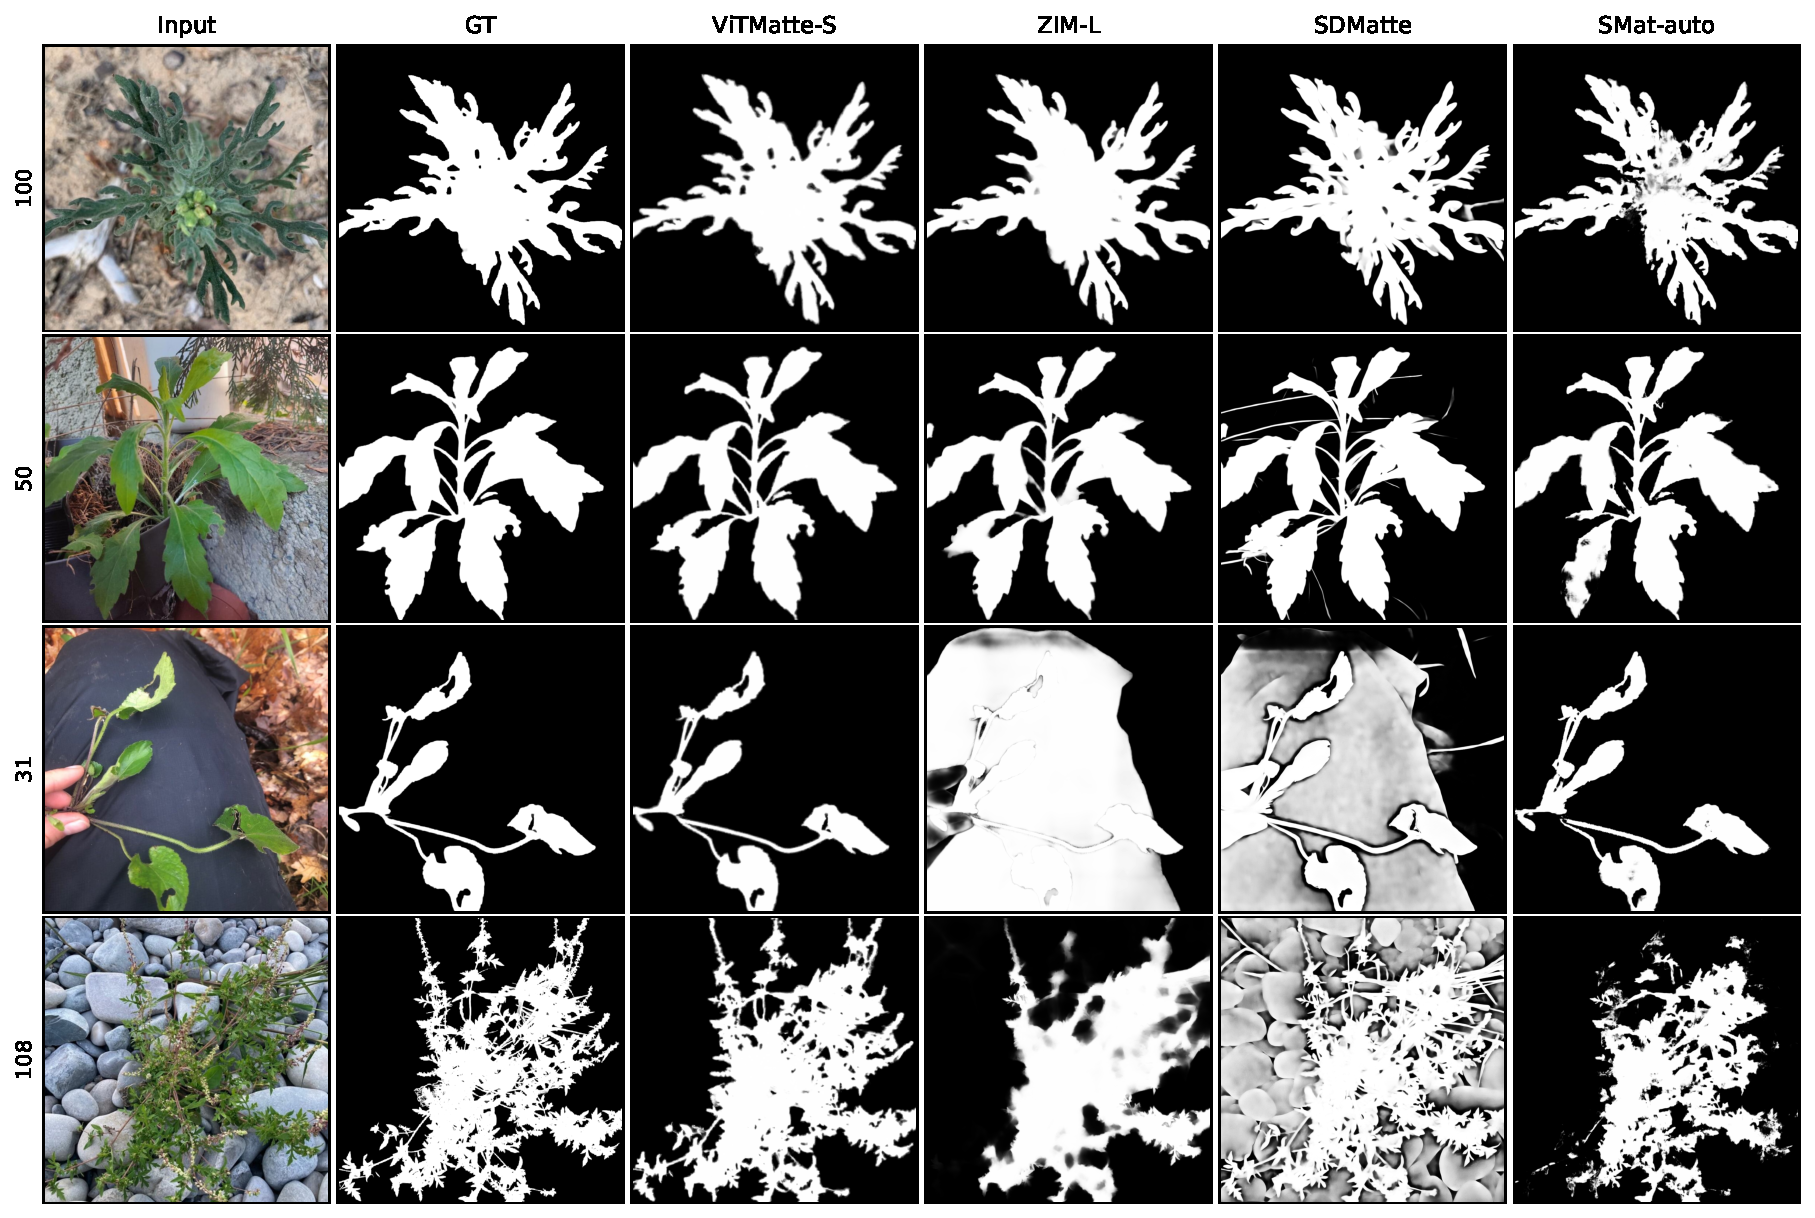
\includegraphics[width=0.98\linewidth]{figures/qualitative.pdf}
		\caption{定性对比（行为样本，列依次为：输入图、真值 alpha、各模型预测 alpha）。上两行为典型样本，下两行（31、108）为主体满框、类内干扰强的难例：ViTMatte 借三分图先验始终贴合真值，而无三分图方法在难例上出现前景范围误判与细节退化。}
		\label{fig:qual}
	\end{figure}

	\subsection{推理效率}
	所有模型均在单张 24\,GB GPU 上完成推理。其中扩散式 SDMatte 在单步推理设置下约 $1.9$\,s/图，SMat 约 $2.3$\,s/图；即便以 Stable Diffusion 2 为骨干，SDMatte 在单卡 24\,GB 内未出现显存溢出。ViTMatte 与 ZIM 推理更轻量（未做系统计时）。可见这些大型预训练抠图模型在单卡条件下均可实用部署。

	\subsection{跨数据集复现自验}
	为确认复现忠实、并区分「模型能力」与「植物域难度」，我们在各模型\emph{原始论文基准}上做了跨数据集自验（表~\ref{tab:crossval}）。其中 ZIM 在其论文提出的 MicroMat-3K 上以官方评测流程运行，SMat 与 SDMatte 在自动抠图基准 AIM-500 上评测（按 AIM 论文~\cite{AIM} 惯例采用全图口径）。各模型在原基准上的数值与表现规律与原文一致（如 ZIM 在框提示下显著优于点提示、且对大目标更难），表明本文复现忠实；对照之下，PM 植物场景上的较高误差应主要归因于数据域特性，而非复现失真。

	% Auto-generated by scripts/generate_table.py -- do not edit by hand.
% Cross-dataset sanity check with paper-reported values for comparison.
\begin{table}[ht]
\centering
\caption{跨数据集复现自验：本文复测值与论文报告值对照。(a) SMat/SDMatte 在 AIM-500(自动抠图基准,500 张,全图口径);(b) ZIM 在其原论文基准 MicroMat-3K(官方 eval pipeline,$\times 10^{-3}$)。SMat 论文未在 AIM-500 上单独报告 point8 指标,故本文 point8 仅作附加自测,不列论文对照。}
\label{tab:crossval}
\setlength{\tabcolsep}{4pt}
\small
% (a) AIM-500
\begin{tabular}{llccccc}
\multicolumn{7}{l}{\textbf{(a) AIM-500 (whole,500 张)}}\\
\toprule
模型 & 来源 & SAD & MSE & MAD & Grad & Conn \\
\midrule
SDMatte (box) & 本文 & 29.35 & 0.0100 & 0.0178 & 24.06 & 15.62 \\
SDMatte (box) & 论文 & 19.45 & 0.0049 & 0.0116 & 20.63 & 12.58 \\
SMat-auto & 本文 & 34.30 & 0.0129 & 0.0203 & 31.49 & 13.98 \\
SMat-auto & 论文 & 34.30 & 0.0129 & 0.0203 & 31.49 & 13.98 \\
SMat-point8 & 本文 & 29.88 & 0.0102 & 0.0176 & 28.68 & 13.72 \\
\bottomrule
\end{tabular}
\\[6pt]
% (b) ZIM @ MicroMat-3K
\begin{tabular}{lllccc}
\multicolumn{6}{l}{\textbf{(b) ZIM-ViT-B @ MicroMat-3K ($\times 10^{-3}$,all scale)}}\\
\toprule
子集 & prompt & 来源 & SAD & MSE & MAE \\
\midrule
fine & point & 本文 & 31.33 & 8.23 & 10.76 \\
fine & point & 论文 & 31.286 & 8.213 & 10.740 \\
fine & bbox & 本文 & 9.92 & 1.89 & 3.41 \\
fine & bbox & 论文 & 9.961 & 1.893 & 3.426 \\
coarse & point & 本文 & 6.67 & 1.79 & 2.33 \\
coarse & point & 论文 & 6.645 & 1.788 & 2.320 \\
coarse & bbox & 本文 & 1.86 & 0.45 & 0.66 \\
coarse & bbox & 论文 & 1.860 & 0.448 & 0.659 \\
\bottomrule
\end{tabular}
\end{table}


	\subsection{结果分析}

\textbf{三分图先验带来的差距。} 由表~\ref{tab:pm} 可见，享有三分图先验的 ViTMatte 在全图口径上明显领先（SAD 25.5、MSE 0.012），因为前景范围已由三分图给定，模型只需在狭窄的未知带上精修；三种无三分图方法则需自主完成前景判定，其全图 SAD 普遍更高（SDMatte 44.3、SMat-auto 64.1、ZIM-L 93.2）。这一差距并非单纯的「模型优劣」，而是输入条件不同的直接体现，正对应「给定前景的精修」与「自主前景选择」两条路线的本质区别。

\textbf{全图与未知区域的分歧。} 值得注意的是，若只看\emph{未知区域}指标，SDMatte（SAD 23.9）甚至略优于 ViTMatte（24.3），说明在边缘细节的局部刻画上，扩散先验与三分图精修旗鼓相当；三种无三分图方法的全图误差主要来自\emph{未知区域之外}的前景范围误判，而非边缘本身。这印证了同时报告两套口径的必要性——全图指标度量「主体识别/图形-背景分离」，未知区域指标度量「边缘细节质量」，二者分离才能定位误差来源。

\textbf{无三分图方法之间的比较。} 三者中扩散式 SDMatte 最稳健，在全部 150 张上零图形-背景反转；SMat 自动模式凭借 DINOv2 显著性前端，零提示即可避免反转，交互（8 点）相比自动几乎无提升，说明其自动分支已抓对前景。相比之下，ZIM 的软 matte 头在「主体满框」的植株上常把更大、更干净的背景区误判为前景，即使给定真值框与 8 个前景点仍会发生图形-背景反转，是其全图误差显著偏高（SAD 93.2）的主因。这说明在植物域，自动前端的前景判定（而非边缘刻画）才是主要瓶颈。

\textbf{定性观察。} 图~\ref{fig:qual} 直观印证上述结论：在典型样本（如第 1 行）上各模型预测均贴近真值；而在主体满框、与背景同种植株相似的难例（第 3、4 行）上，无三分图方法出现前景范围扩张或细枝丢失，ViTMatte 则因三分图约束始终稳定。结合跨数据集自验（表~\ref{tab:crossval}）中各模型在通用基准上的良好表现可知，植物场景的困难主要来自数据域本身的图形-背景模糊性，而非模型在边缘刻画上的不足。


	\section{结论与讨论}
	本文在统一协议下复现并对比了四种范式的抠图方法。主要结论为：(1) 在给定三分图先验时，ViTMatte 取得最佳的全图精度（SAD 25.5），印证「给定前景下的精修」相对容易；(2) 在三种无三分图方法中，扩散式 SDMatte 最稳健（全图 SAD 44.3、零图形-背景反转），SMat 自动模式次之且零提示即不反转，而 ZIM 软 matte 头在满框植株上易发生图形-背景反转，是其误差偏高的主因；(3) 跨数据集自验表明各模型复现忠实，植物场景的较高误差主要来自主体满框与类内相似干扰等数据域特性。

	\textbf{各范式的适用性与认知启示。} 当能够获得可靠三分图（或可由交互廉价生成）时，三分图精修路线在植物细结构上最稳；当要求全自动时，具备强语义先验的自动前端（SDMatte 的扩散先验、SMat 的 DINOv2 显著性）比 SAM 式软 matte 头更能完成「图形-背景分离」。这与视觉认知的直觉一致：当目标边界由外部「自上而下」给定时，系统只需专注局部细节；而要「自下而上」自主分离前景时，是否具备充分的语义/对象先验，直接决定了在同质场景下能否正确选中目标。ZIM 在满框植株上的系统性反转，正是「自主目标选择」机制在缺乏对象级先验时的失败缩影。

	\textbf{局限与展望。} 受篇幅与范围所限，本文为复现与定量对照工作，尚未展开系统的 failure case 归类（如主体识别失败、前景范围误判、类内相似干扰、细结构丢失等）与认知挑战样本标注；这些是把定量结果与认知机制进一步打通的关键，留作后续工作。此外，可针对 ZIM 的图形-背景反转这一系统性失败设计轻量后处理或提示策略改进，并在同协议下做前后对比。

	\bibliography{Bibs/reference.bib}
\end{document}
